\documentclass[letterpaper, 10 pt,conference]{ieeeconf}  % Comment this line out if you need a4paper

%\documentclass[a4paper, 10pt, conference]{ieeeconf}      % Use this line for a4 paper

\IEEEoverridecommandlockouts                              % This command is only needed if 
                                                          % you want to use the \thanks command

\overrideIEEEmargins                                      % Needed to meet printer requirements.

% See the \addtolength command later in the file to balance the column lengths
% on the last page of the document

% The following packages can be found on http:\\www.ctan.org
\usepackage{graphicx} % for pdf, bitmapped graphics files
\graphicspath{{../}}
\usepackage{epstopdf} % for postscript graphics files
\usepackage{mathptmx} % assumes new font selection scheme installed
\usepackage{times} % assumes new font selection scheme installed
\usepackage{amsmath} % assumes amsmath package installed
\usepackage{amssymb}  % assumes amsmath package installed
\usepackage[caption=false,font=footnotesize]{subfig}
\usepackage{fixltx2e}
\usepackage{float}

\title{\LARGE \bf
3D-PIV application for autonomous vehicles using monocular vision
}


\author{Eduardo da Silva Afonso$^{1}$ and Fernando Pujaico Rivera$^{2}$ and Arthur de Miranda Neto$^{3}$% <-this % stops a space
\thanks{The authors are with Terrestrial Mobility Lab. at the Federal University of Lavras, Lavras - MG, Brazil.}%
\thanks{$^{1}$  eduardo.afonso@engautomacao.ufla.br, $^{2}$  201518201@posgrad.ufla.br, $^{3}$  arthur.miranda@deg.ufla.br}%
}

\begin{document}


\maketitle
\thispagestyle{empty}
\pagestyle{empty}

\begin{abstract}

In this paper, the Particle Image Velocimetry ($PIV$) technique was adapted to be used in autonomous vehicles.
Applying PIV and the Pearson’s Correlation Coefficient, our proposed algorithm 
is capable of making a three dimensions tracking of the target possible (Region Of Interest) $ROI$ 
and generates a relative departure factor. These data are used to estimate the 
relative velocity of the target ($ROI$) and then analyse the collision risk.

\end{abstract}
\section{INTRODUCTION}

Traffic accident has been an important point to government. The world average of people
died at traffic is around 10 people per 100 thousand, but in countries, like Brazil, it can be worse.
In 2016, the group which compose the UN General Assembly adopted a resolution for
improve global road safety and they consider that 2011-2020 is Decade of Action for Road Safety.
Traffic jam is other problem faced by cities, it is caused by reckless drivers and accidents.
Many centers of research have been studying solutions to improve this condition and decrease the 
numbers of death and accidents.

Monocular vision comes is an emerging field in autonomous vehicles. 
Several application have presented solutions to current problems, 
however systems  of low computational cost remain a challenge. 


The Particle Image Velocimetry ($PIV$)\cite{Bastiaans} technique is used in many fields of 
knowledge, \cite{Story, Xu}, to calculate the velocity of fluids in different parts. 
Here, $PIV$ was adjusted for the case of autonomous vehicles using matching criteria based on 
the Pearson Correlation Coefficient ($PCC$)\cite{Miranda Neto} over the KITTI dataset\cite{Geiger}.

Here, we define some variable used in the paper. The object of interesting is called target.
The region of interesting (ROI) is part of image where the target is and
Window of Search (WOS) is a rectangle where the program will search the ROI. 




\section{THEORETICAL FOUNDATION}

\subsection{THE PEARSON CORRELATION COEFFICIENT}

$PCC$ is used in statistical analyses, pattern recognition and computer vision. 
It can be used to comparing two images in an object recognition system. 
The following equation describes the $PCC$ method for two gray scale digital images\cite{Eugene},
represented by the matrices $A$ and $B$ with $M$ elements each one,
\begin{equation}
r = \frac{\sum \limits_{i}^{M} (a_i-\mu_a)(b_i-\mu_b)}{\sqrt{\sum \limits_{i}^{M} (a_i-\mu_a)^2} \sqrt{\sum\limits_{i}^{M} (b_i-\mu_b)^2}}.
\end{equation}

where $a_i$ is the intensity of the i-th pixel in the  matrix $A$, 
$b_i$ is the intensity of the i-th pixel in the matrix $B$, 
$\mu_a$ is the mean intensity of $A$,
$\mu_b$ is the mean intensity of $B$ and
$r$ is the correlation coefficient \cite{Miranda Neto}.


\subsection{PARTICLE IMAGE VELOCIMETRY}

$PIV$ is a technique to determine a velocity field from a stream of consecutive 
images of seeded flows\cite{Bastiaans}.
This result is given as a vector field, demonstrating direction, sense and 
intensity of velocity in each particle. 
Moreover, it is possible to calculate rapidly the velocities of any part of image.
For this purpose, the $PIV$ technique divides the image in analysis regions (particles), 
and are searched similarities to these particles in the next image; 
when matches are found, displacement vectors (vector field) are returned,
the analysis regions are refresh and the process is repeated with the consecutive image.



\section{SYSTEM DESCRIPTION}
The purpose of our algorithm is to make a three dimensions tracking system, producing position informations 
about a followed target.
The information will be relevant to define parameters 
as: the relative velocity, the factor of approaching and of departure.

The proposed algorithm is shown in Fig. \ref{fig:system};
it begins with a key frame image where a initial target ($ROI$) is determined; 
the system then receives a stream of image frames and the tracking system 
enters into looping follow this target in the next frames.

\begin{figure}[bhp]
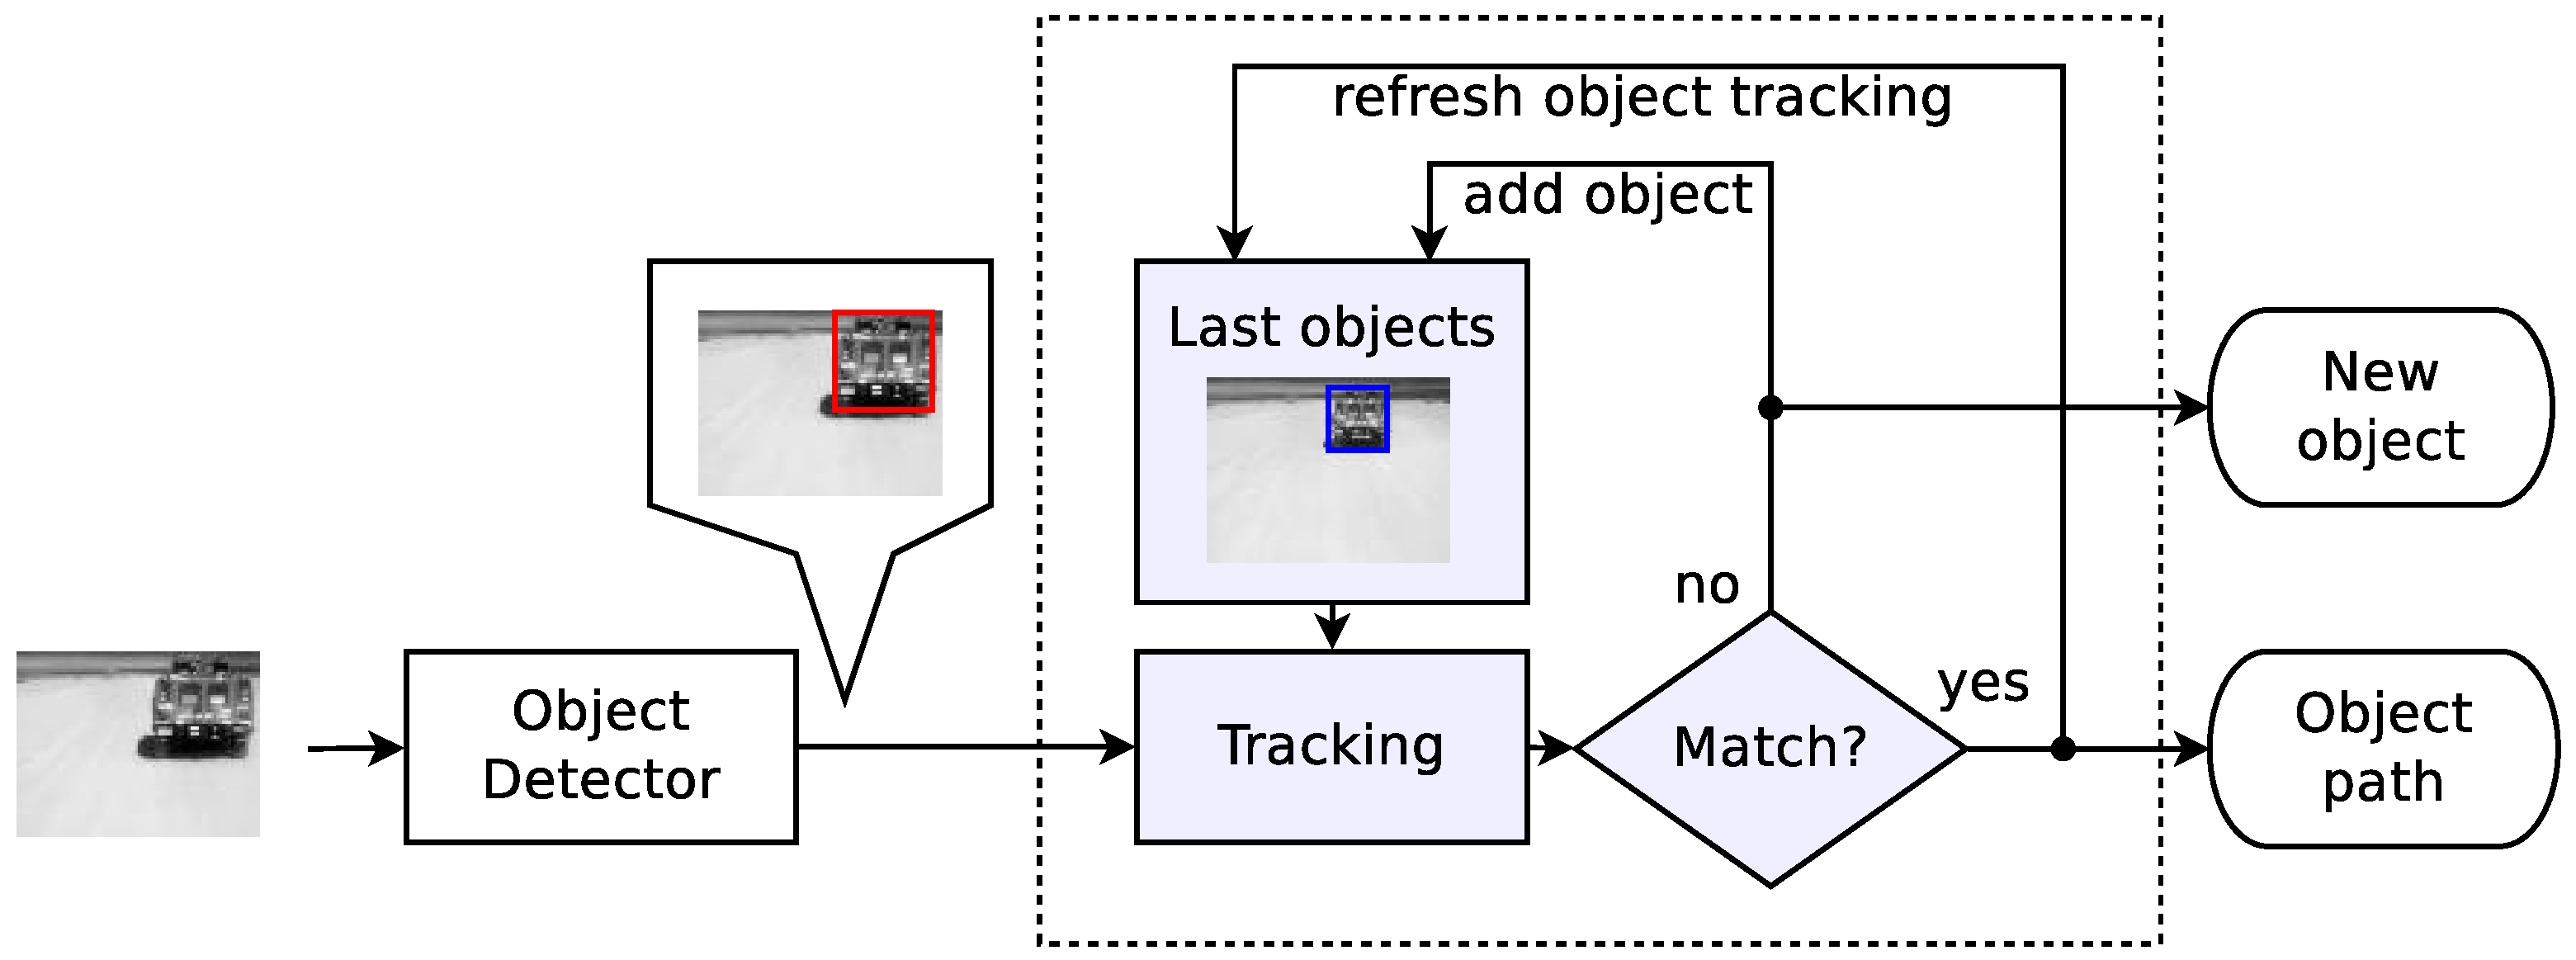
\includegraphics[width=\columnwidth]{images/figure1-diagram1.eps}
\caption{The target is identified from a highest value of correlation (PCC) between a selected ROI and an analysis region in
the $WOS$ of a current frame; the result of this process is a displacement which is  returned as vector field.}
\label{fig:system}
\end{figure}

In a two dimensional analysis, the tracked target given us information about its horizontal 
and vertical position and it is relative to the perpendicular velocity with respect to the observer.
When the target is analyzed in three dimensions, 
the initial $ROI$ has the position $(x=x_0,y=x_0,d=d_0=1)$;
where, $x_0$ and $y_0$ represent a position (horizontal and vertical) in the analyzed image,
and $d_0=1$ represents the initial depth position of target in the $ROI$ (normalized by definition to $1.0$).
Thus, all the results of depth will be relative to this value. In this sense, the relative velocity and 
the factor of approaching or departure can be calculated.

%Diagrama1
 %A gente vai explicar o algoritmo como uma caixa fechada , que coisa entra e que coisa sai
 %e os parametros a sintonizar.
 % como usar ele quando implementado, como se fosse uma caixa preta.


\section{ALGORITHM DESCRIPTION}
 
%DiagramaX

\subsection{MULTI-RESOLUTION MATCH CRITERIA}
Method to track object at image is based on PIV. Figure 2(a) shows the application in 2 dimensions and the next in
3 dimensions.

\begin{figure}[H]
\centering
  \subfloat[]{\label{subfig:(a)} 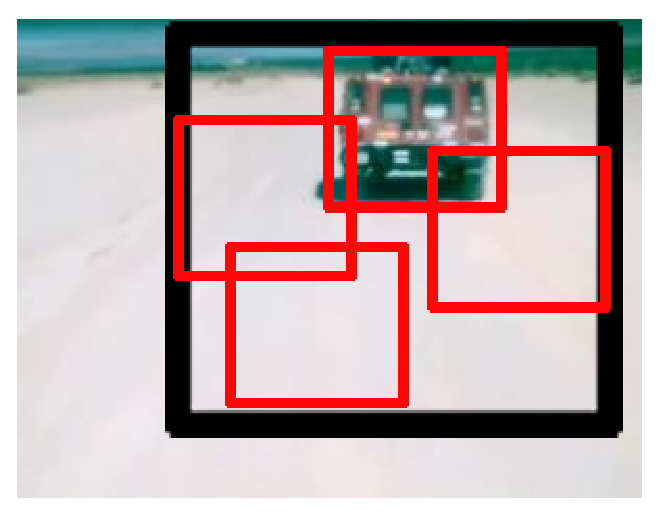
\includegraphics[width=.5\columnwidth]{images/figure2a.eps}}
  \subfloat[]{\label{subfig:(b)} 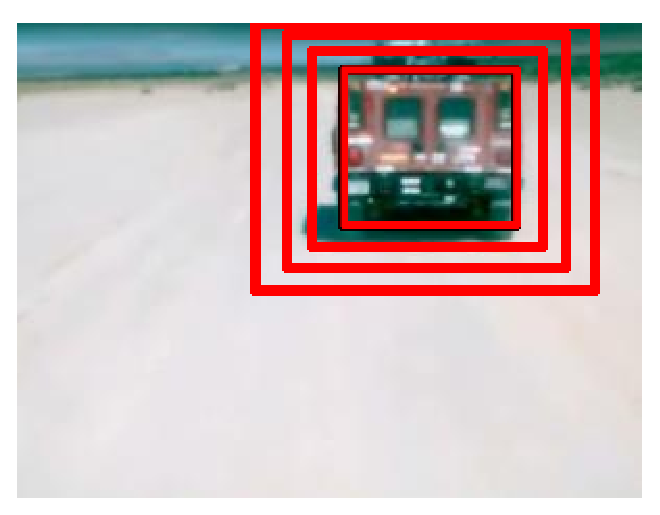
\includegraphics[width=.5\columnwidth]{images/figure2b.eps}}
  \caption{The red box in figure (a) shows the ROI and black box is WOS. In the figure (a), 
  ROI is compared with first portion on the left top of WOS, and these comparisons are made 
  pixel by pixel for whole WOS. The black boxes, in the figure (b), are the WOS used 
  to different layers of search in 3 dimensions}
\end{figure}

To track the object, the ROI defines the size of WOS and, verify the similarity of ROI and parts of WOS using PCC. 
The highest coefficient of Pearson determines new place of object. The figure 2(b) reveals how the dimension of depth was included and, 
the search is made in different layers. In 3 dimensions, the target also is found from the highest PCC among WOS, but the object may be 
bigger or smaller, depending in which layers was.\\
%onde estava, onde esta agora
%que tamanho tinha que tamanho tem.
\subsubsection{MULTI-SCALE 3D INTERPRETATION}
To understand this technique we need to analyse the same target in 
two different positions, as in Fig. \ref{fig:multiscale3d}.

\begin{figure}[H]
\centering
  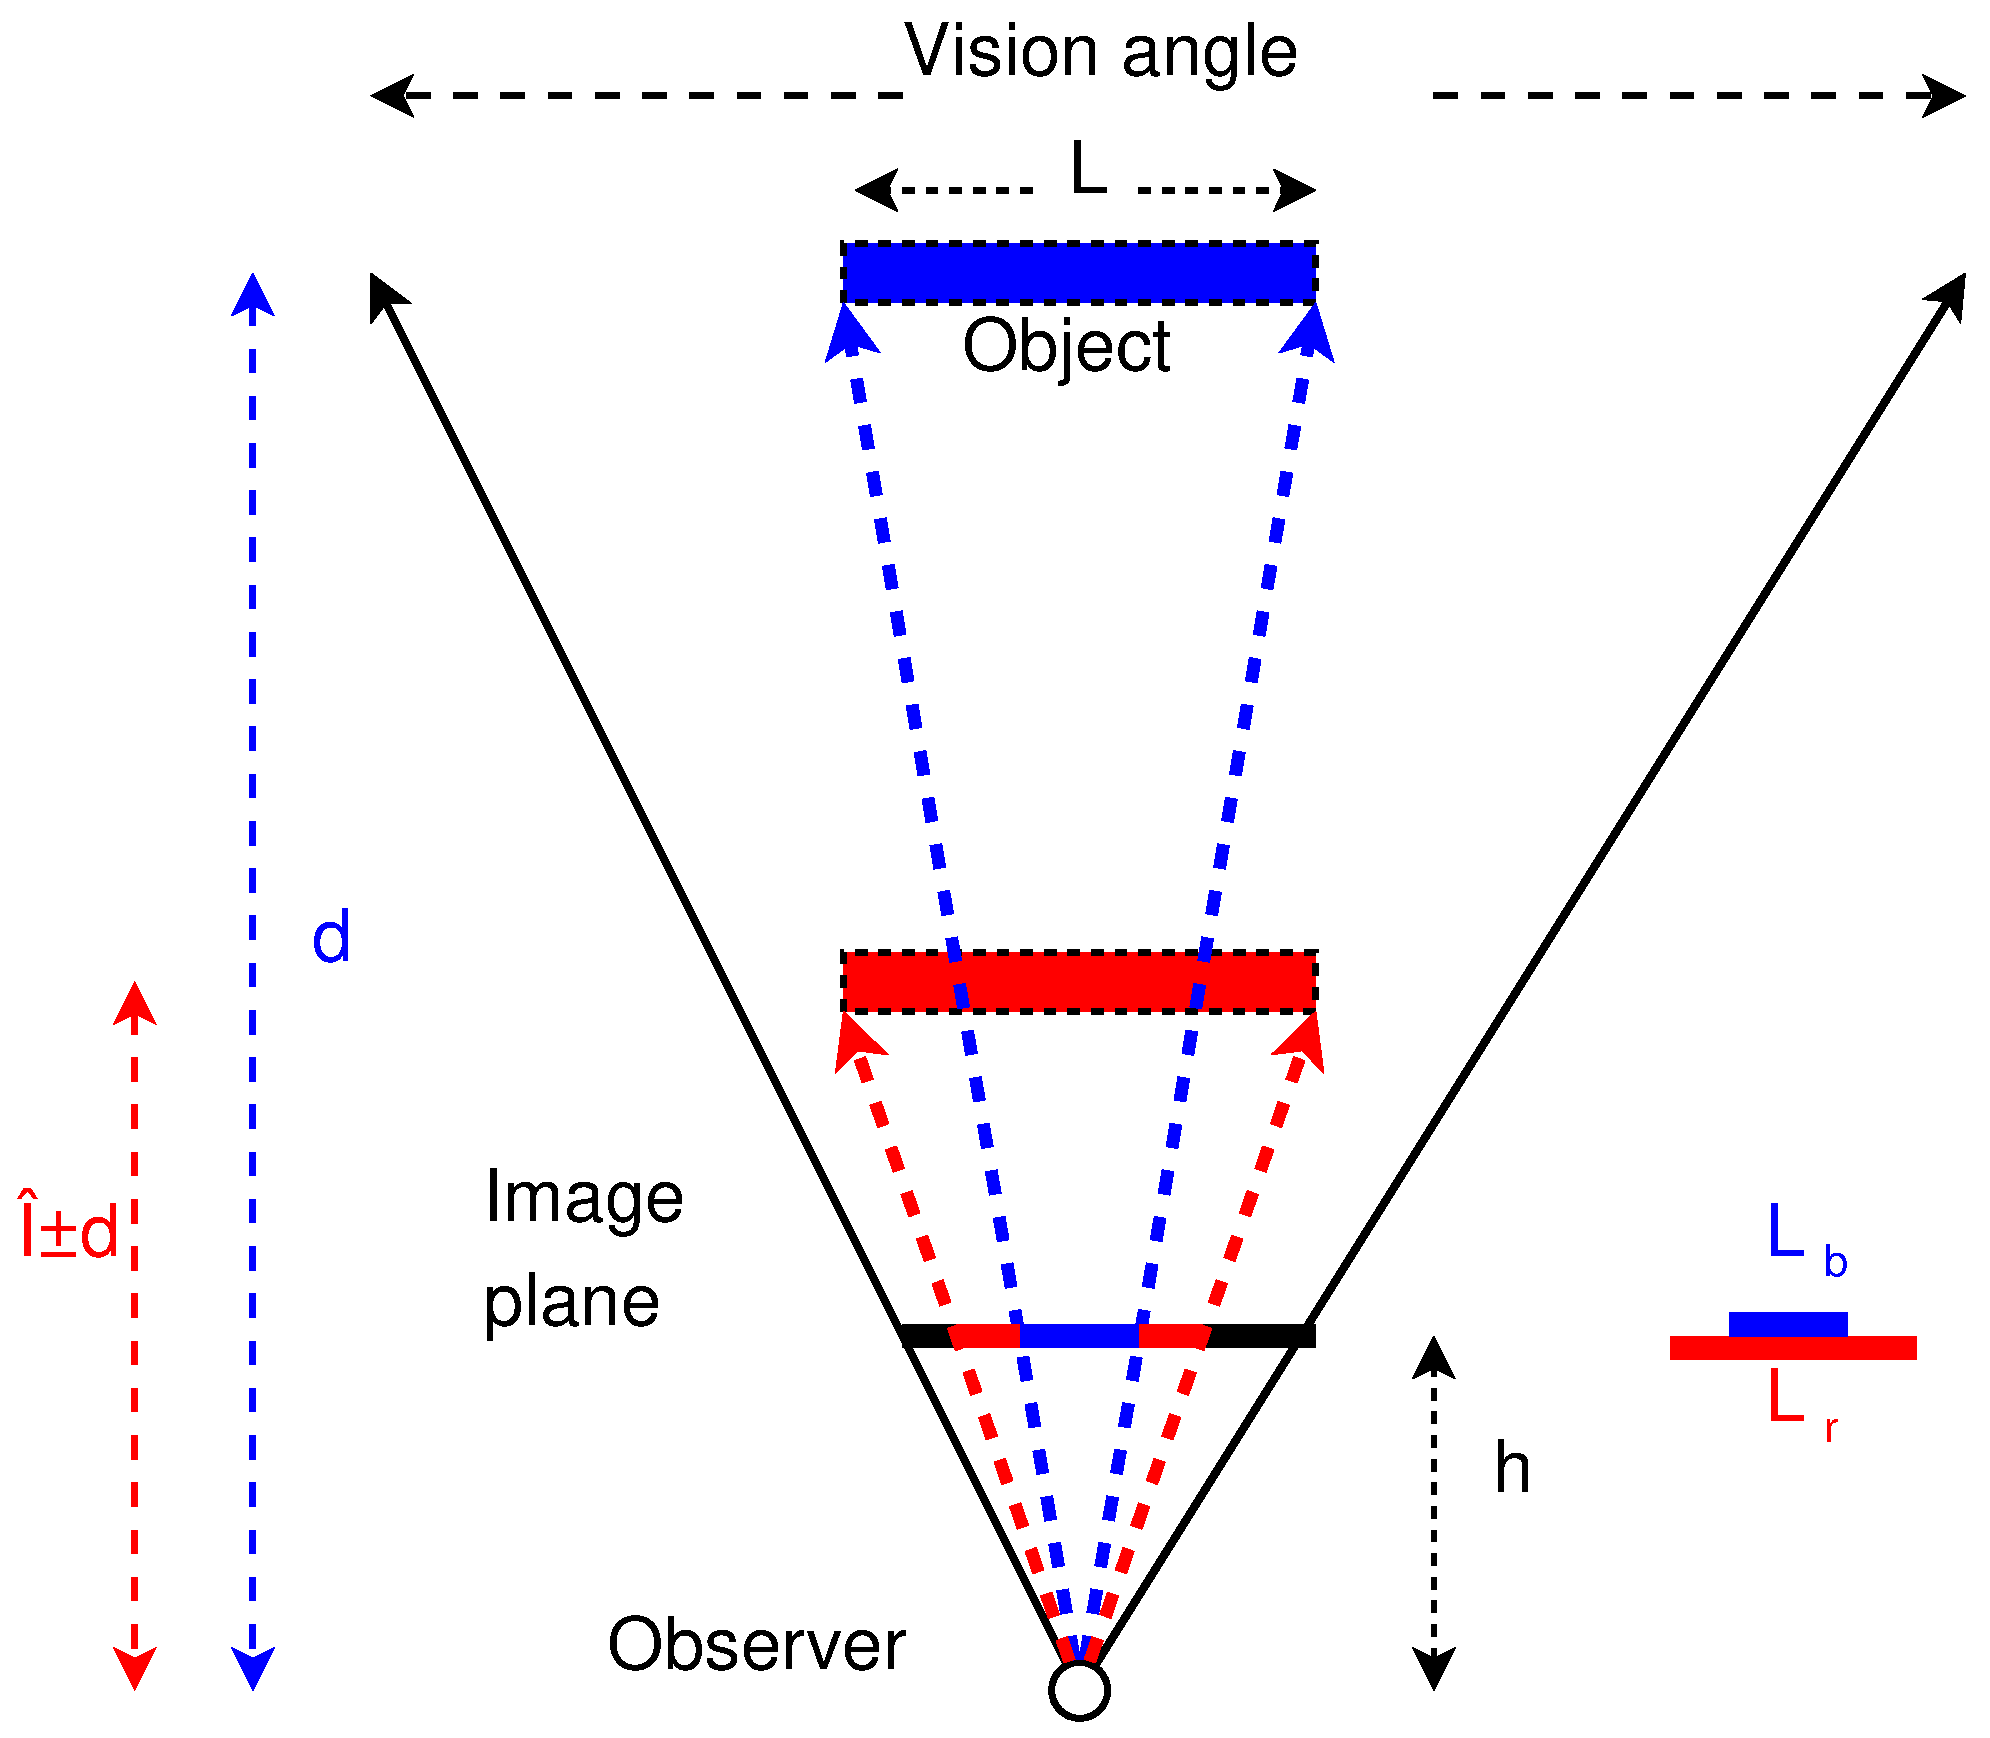
\includegraphics[width=.7\columnwidth]{images/Diagrama3.eps}
  \caption{The multi-scale tracking.}
  \label{fig:multiscale3d}
\end{figure}

Fig.\ref{fig:multiscale3d} shows the same target at two different distances $d$ and $\alpha d$, respectively, in blue and red.
The image plane is located at a distance $h$ of the observer.
The projections of objects, in blue and red, are labelled in the image as
$L_b$ and $L_r$, respectively. Making a simple inspection in the
formed triangles, we can see that $\frac{h}{d}=\frac{L_b}{L}$ and 
$\frac{h}{\alpha d}=\frac{L_r}{L}$, then $L_b/\alpha= L_r$. 
From the point of view of the observer, this implies that when a target 
is located at a distance $d$ at a time $t_0$,  and a distance $\alpha d$ at a time $t_1$, 
the width of the target in the image plane is altered by a factor of 1/$\alpha$, 
and consequently its area is altered by a factor of 1/$\alpha^2$.

The criterion method the searches for objects using different discrete values of $\alpha$. 
The algorithm tracks the nearest objects with $\alpha<1$ and objects farthest with $\alpha>1$.

%usa Multi-resolution match criteria e explica isso dos tamanhos

\subsubsection{DEPARTURE FACTOR - RELATIVE VELOCITY}
The departure factor is a dimensionless number related to the rate of approach 
or departure of a target to the observer. The factor
is determined in \ref{eq:relarea},

\begin{equation}\label{eq:relarea}
f_a \equiv \alpha^2 \equiv \frac{Area_r}{Area_f} 
\end{equation}

where $f_a$ and $\alpha$ are defined as factor area and departure factor, 
respectively; $Area_r$ is the ROI area and $Area_f$ 
is the analyzed region in the current image frame.

Thus, knowing $\alpha$, if we consider that the target in the $ROI$ was to a distance $d_0$,
then the target in the analysis region will be to a distance of $\alpha d_0$ (or $\sqrt{f_a} d_0$).
So that, each $i-th$ frame will have its own $\alpha_i$ value; where, $d_i=\alpha_i d_0$.

The departure factor, $\alpha_i$, has two interpretations: if the rate of departure increases quickly, 
this  means that the target is departing. If the factor decreases, the 
target is approaching.

The relative velocity is using a simple equation of kinematic in physics:
\begin{equation}
 v_i = \frac{\Delta s}{\Delta t}= \frac{s_i-s_{i-1}}{\Delta t}.
\end{equation}

where the vector $v_i$ represents the relative velocity in the i-th image frame, 
$s_i=(x_i,y_i,d_i)$ is the position of match in the i-th image frame
and $\Delta t$ is the sampling time between image frames.
Additionally, we call velocity of departure factor, $v^d_i$, 
the scalar number which represents the depth component
of the vector $v_i$.

The calculated  $v^d_i$ value is relative, for the simple reason that the distance (depth) between the 
camera (observer) and the target in the instance i-th will be referenced to $d_0$, 
given that the distance of the initial $ROI$ is established by definition to 1.
Finally, in all cases, the position $s_i$ is relative to the observer (a moving reference system).


\subsection{RENEW ROI CRITERIA}
%Diagrama2
The $ROI$ is an important element in the algorithm, because of that this  
will be used as pattern to find a match of tracked object at the current image. 
The  question in this case is to know the best moment to refresh the $ROI$
with a new perspective of object. 
Here, we establish the criteria that when the comparison of images return 
a $PCC$ lower than $0.925$ and greater than $0.8$, then the $ROI$ is changed with the current 
analyzed region and a new position of $ROI$ is establish with $(x_i,y_i,d_i)$. 
Thus, it was adopted as $0.8$ the lower limit to a match case\cite{Eugene},
see Fig. \ref{fig:newroicri}. Values less than $0.8$ cause a  lost object alert.
Finally, it is important to note that if the $ROI$ is changed the new $ROI$ is establish
with the real size of the analyzed region and not with the rescaled version used
in the calculus of the $PCC$.


\begin{figure}[H]
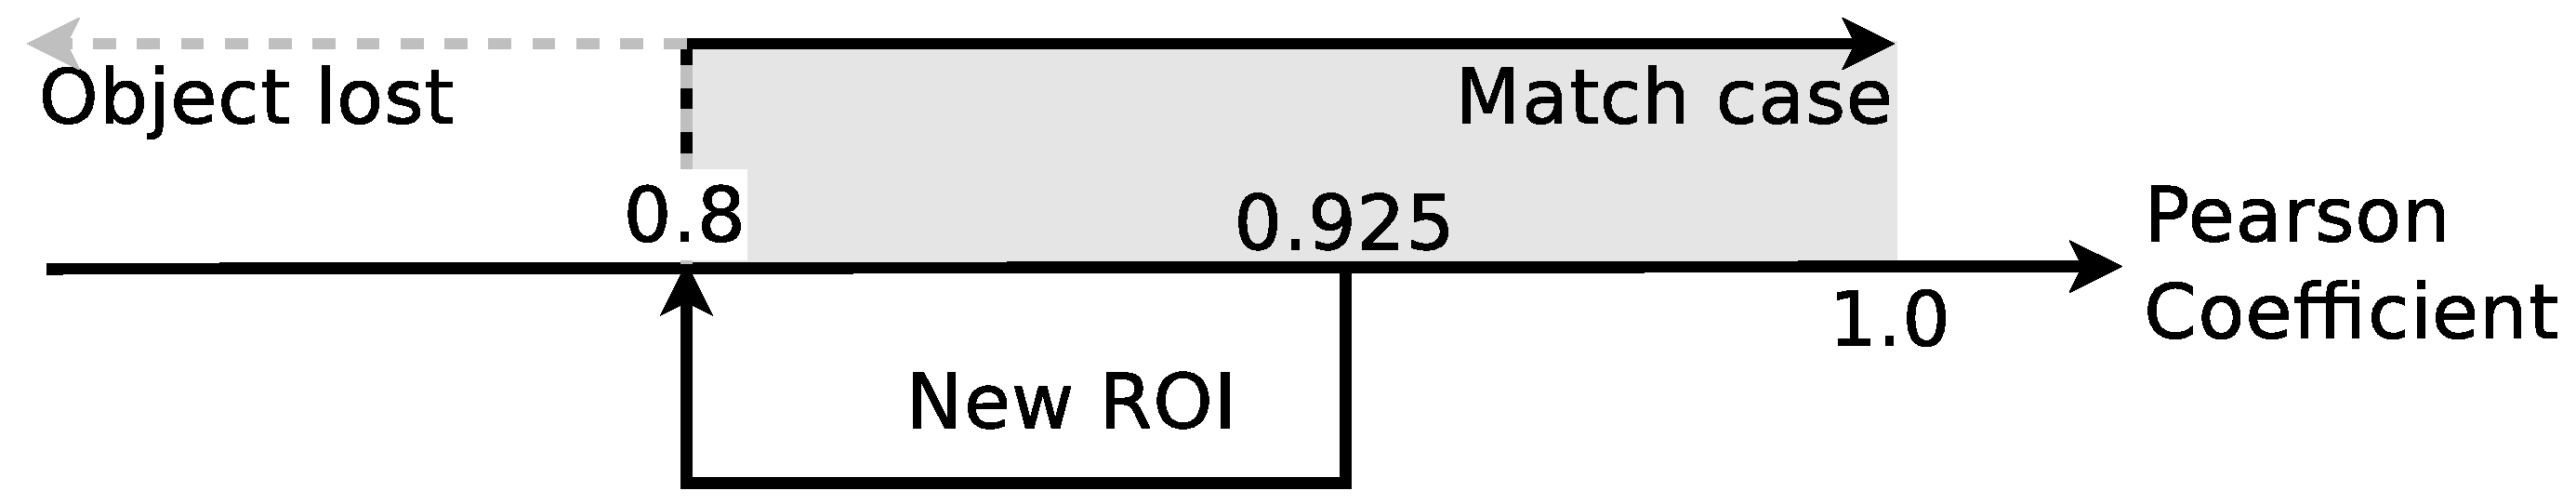
\includegraphics[width=\columnwidth]{images/figure3.eps}
\caption{When the comparison is greater than $0.8$, including numbers bigger than 
$0.925$, means that the target was matched. But if two regions are compared 
and the $PCC$ is less than $0.925$ and greater than $0.8$, 
then the $ROI$ changes to the current analyzed region.}
\label{fig:newroicri}
\end{figure}

The system needs to have high level of reliability, so that the lower limit adopted 
contributes to an operation with minimum of mistakes.

\subsection{ERROR REDUCTION}

In this section, we discuss about the error in analysis of the images. In this sense,
we can see that, the targets have different forms; however, 
a $ROI$ ever will have a rectangular form, so that certain areas will be more important of identify inside of $ROI$.
In Fig. \ref{fig:erroridentified}, there are some areas close of edges that target not occupies; they are
considered like error areas.

\begin{figure}[H]
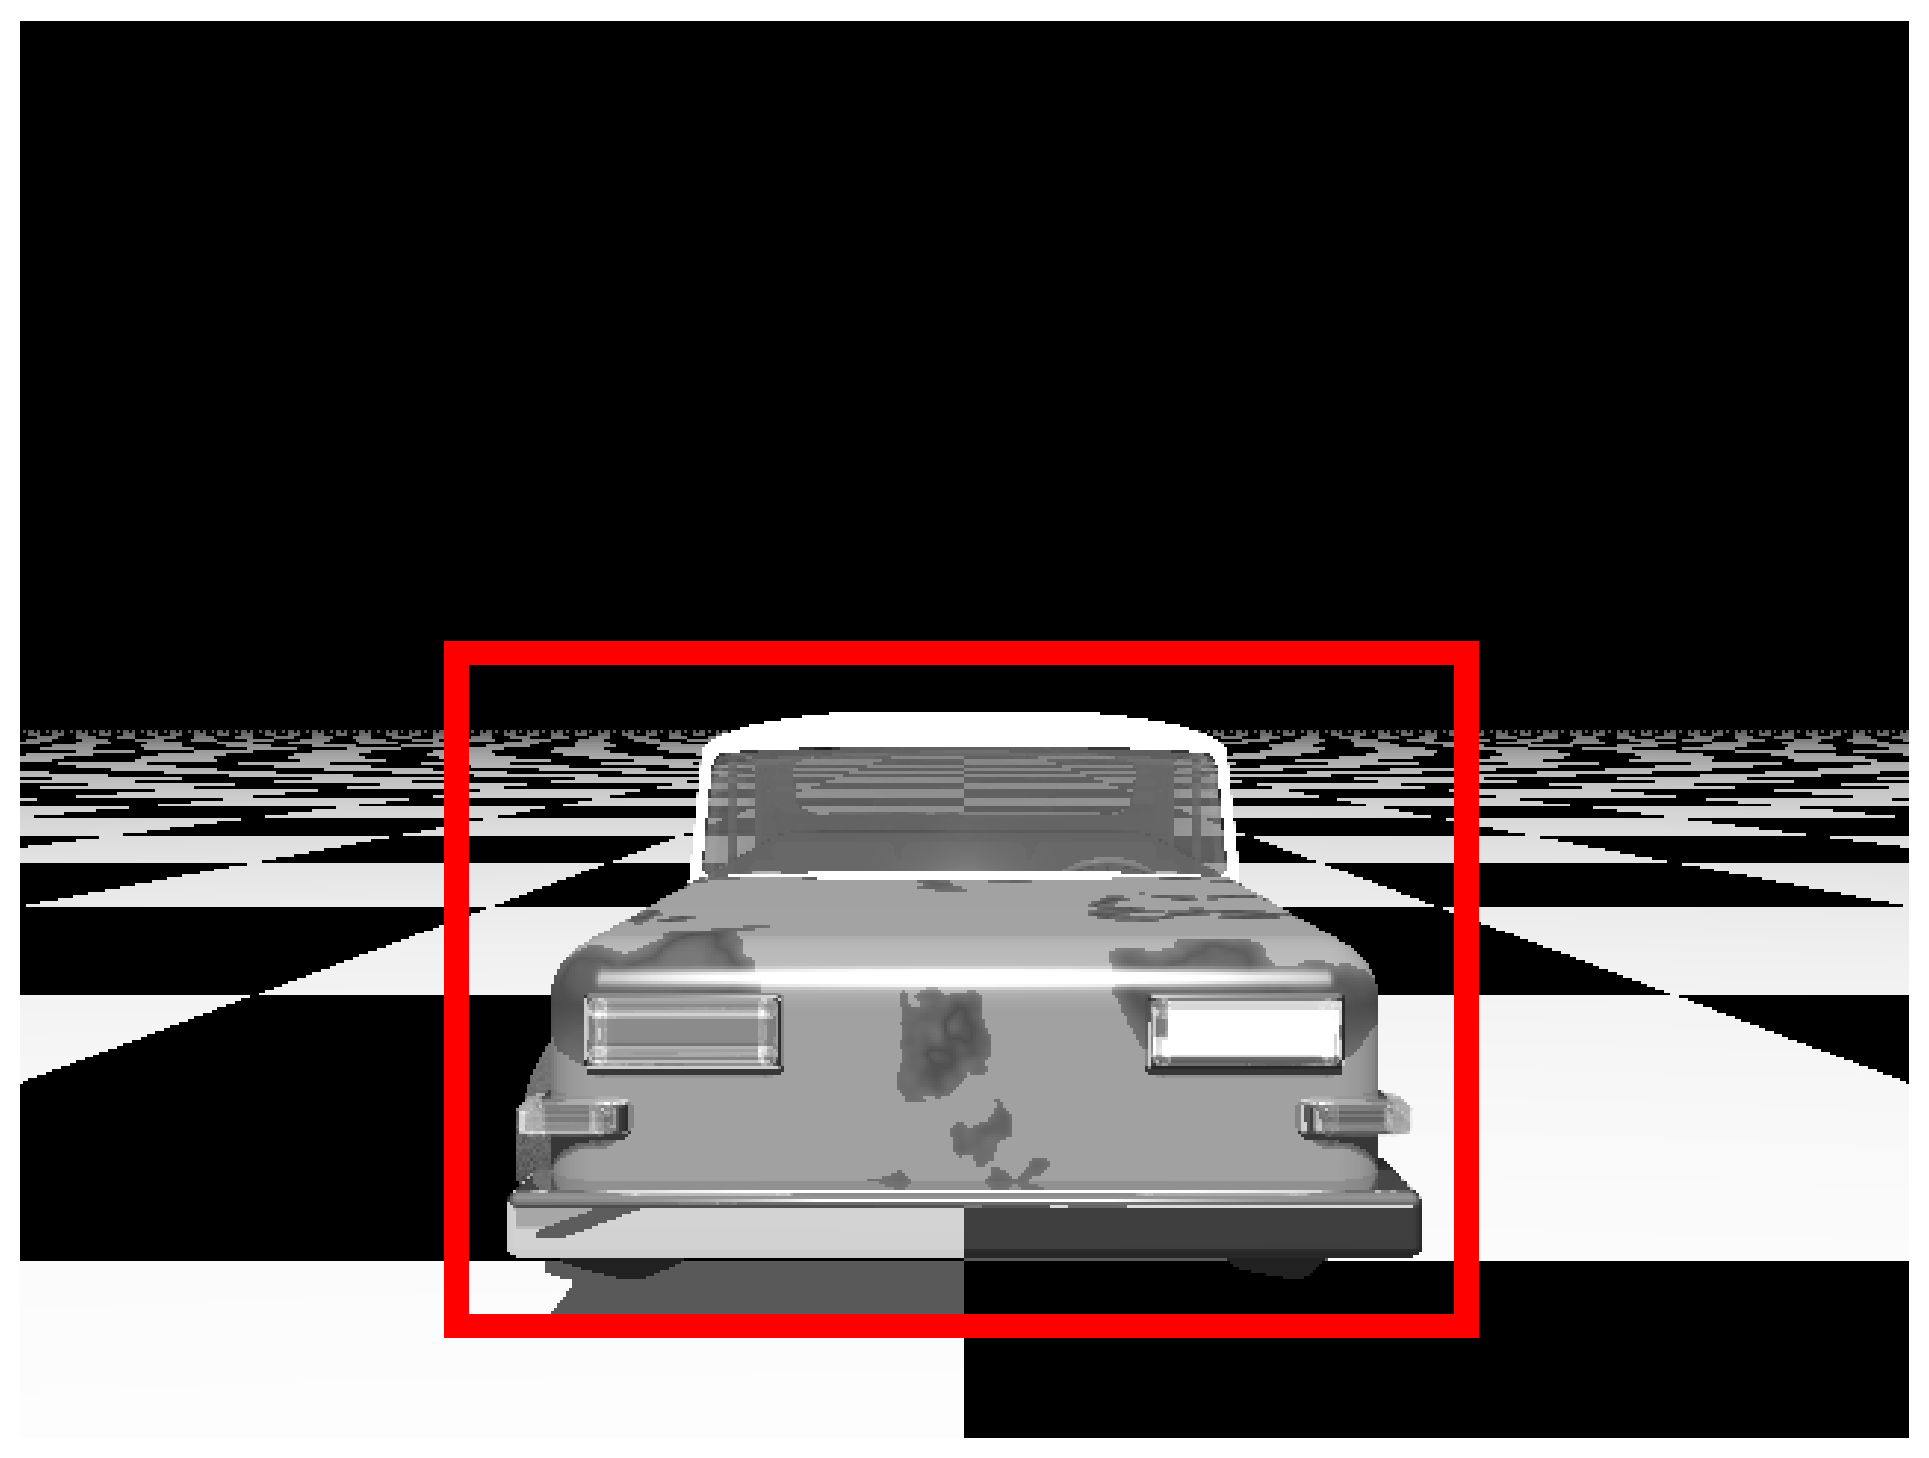
\includegraphics[width=\columnwidth]{images/imageError.eps}
\caption{Illustration of $ROI$ with error areas close of edge.}
\label{fig:erroridentified}
\end{figure}

Whereas, two matrix with the same dimensions can be compared using $PCC$; 
this method of comparison doesn't generate information over the equality of the frames,
but It shows if the frames have a proportional changes for pixel values in the same position. 
Thus, if we consider a high percentage of error area when we compare the frames, It may cause 
decreasing of the correlation level between frames and will given us a fake impression that the target is out of scene.  
We decide solve this problem using a weighting matrix mask over the analyzed regions, 
before the calculus of $PCC$. This can be seen in the Fig. \ref{fig:errorpondered}.
\begin{figure}[H]
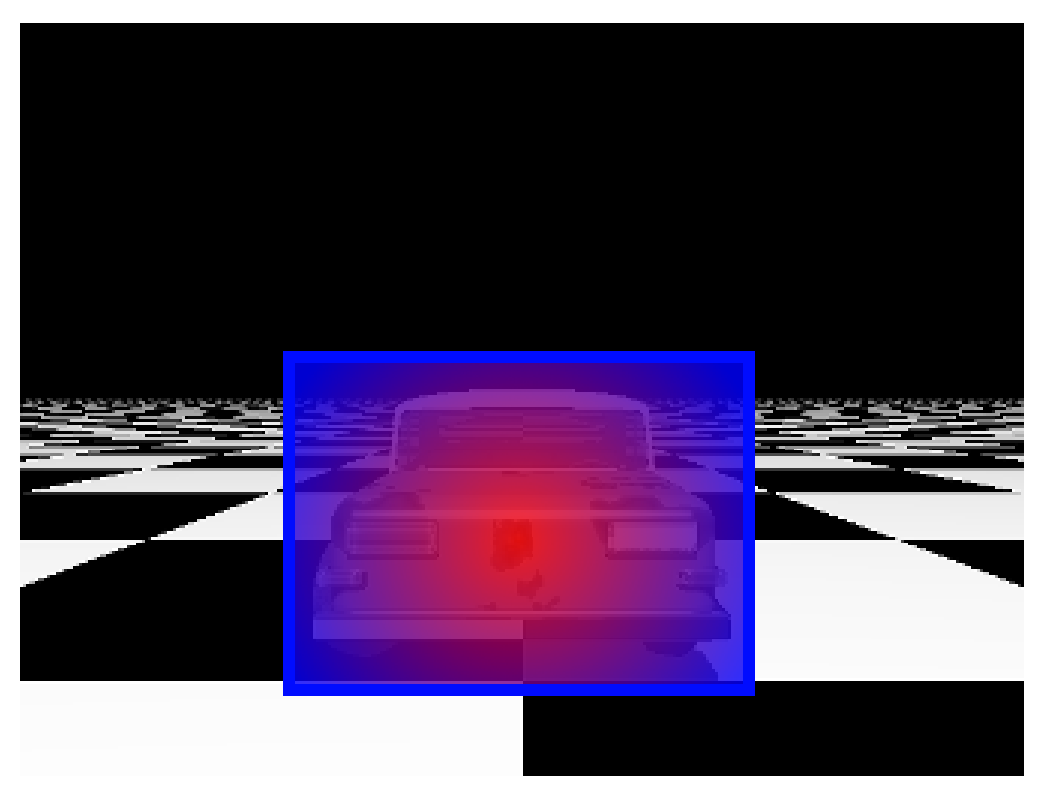
\includegraphics[width=\columnwidth]{images/imageErrorcontroled.eps}
\caption{Illustration of points of most importance (red) and points less importance (blue) in correlation.}
\label{fig:errorpondered}
\end{figure}
Where, points close of edge (in blue color) are considered of less importance, 
points close of center of image (in red color) probably are on the target, and consequently
these points are considered with more importance. 

Thus, to create a weighting matrix mask $Q$ like the seen in the Fig.\ref{fig:errorpondered},
we calculate the $Q(x,y)$ value as showed in the Eq. (\ref{eq:Q}), 
\begin{equation}\label{eq:Q}
 Q(x,y) = \sqrt{e^{ -\frac{|x-\mu_X|^3}{\sigma_X^3}-\frac{|y-\mu_Y|^3}{\sigma_Y^3}  }},
\end{equation}
where $Q(x,y)$ represents a value, in the line $x$ and column $y$,
$\mu_X=H/2$, $\mu_Y=W/2$, $\sigma_X=H/3$ and $\sigma_Y=W/3$; being $H$ and $W$
the height and the width, respectively, in the matrix (analysis region).

Finally, similarly to seen in the Eq. (\ref{eq:PCC}), we multiply the matrix $Q$, 
element by element, over the analysis regions
$A$ and $B$ to calculate the $r_Q$ weighted correlation coefficient, 
\begin{equation}\label{eq:rw}
 r_Q = PCC(Q~A, Q~B).
\end{equation}




% descrição do sistemA
\section{EXPERIMENTAL RESULTS}
The followed informations introduce the results of two different tests 
using POV-Ray.

In the first test, Fig. \ref{fig:imgpapercerta}, 
the algorithm makes the tracking of an object through 14 images in sequence with 
a horizontal displacement to the camera.

\begin{figure}[H]
\centering
  \subfloat[]{\label{fig:imgpapercertaa} 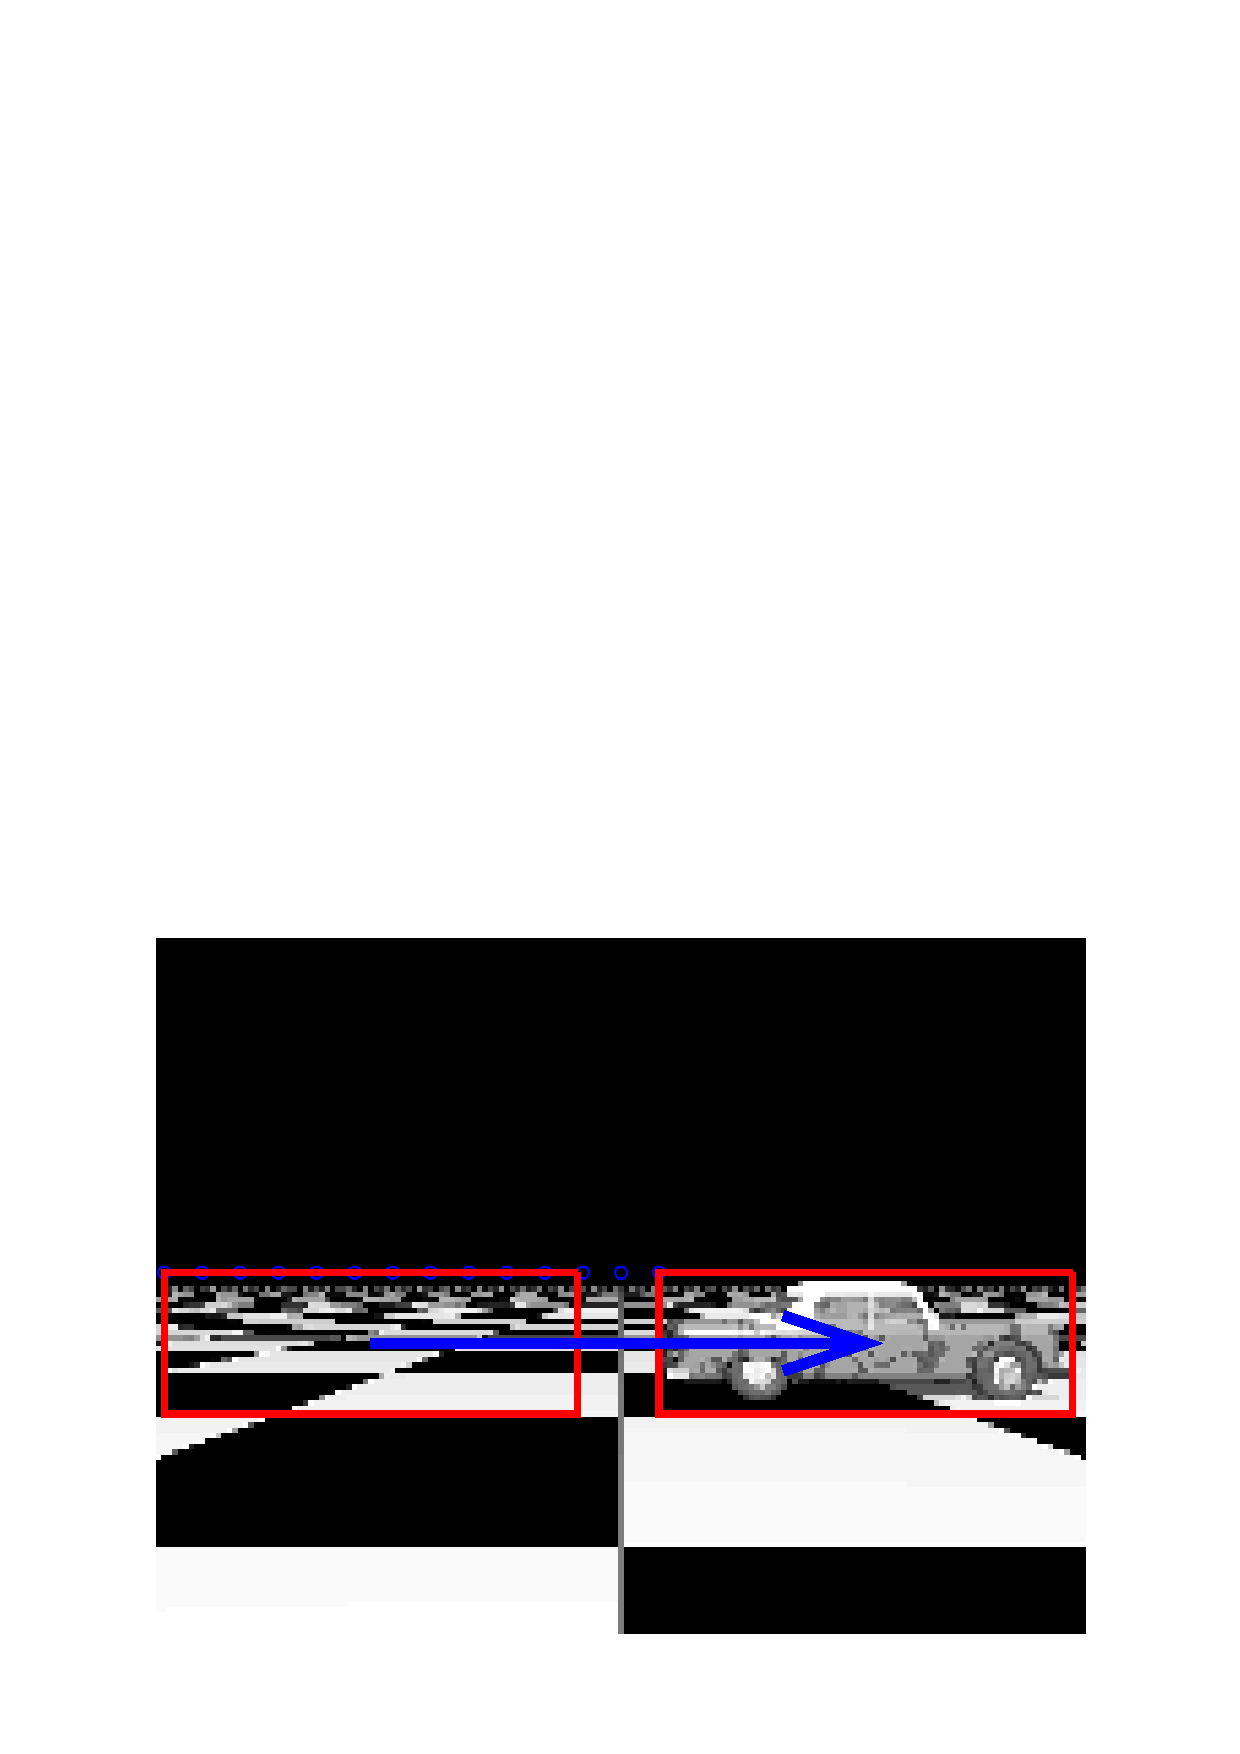
\includegraphics[width=.48\columnwidth]{images/results_2D.png}}
  \subfloat[]{\label{fig:imgpapercertab} 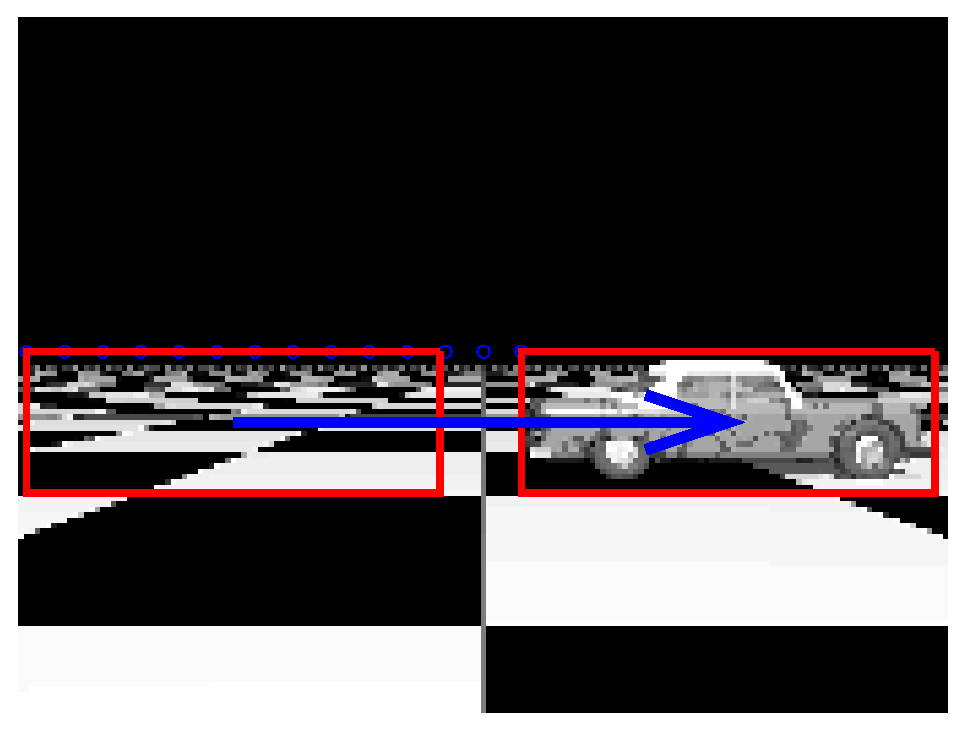
\includegraphics[width=.48\columnwidth]{images/results_2D.eps}}
  \caption{The image in (a) represents the target in its initial position 
   and the image (b) shows the vehicle in its final position.}
  \label{fig:imgpapercerta}
\end{figure}

The initial position of target is in the image (a) and the final position in (b), 
where a vector (in blue) illustrates the resulting trace.
We can observe that there is a small bend in the image 
and it generates a slight change of object perspective. 
The update of the $ROI$ is frequently done, which involves seeing a slight change in area.
The difference between the initial and final values of the departure factor may 
be considered constant, and the value is 1. It means that image doesn't approach to the camera
%as shown in Fig. \ref{fig:res_graph1}.

%\begin{figure}[H]
%\centering
%\includegraphics[width=0.8\columnwidth]{images/results2D_graph.eps}
%\caption{Departure factor for each frame in the test 1.}
%\label{fig:res_graph1}
%\end{figure}

%Fig. \ref{fig:res_graph1v} shows 
The value of the velocity of departure factor is $d_0=1$ and $\Delta t=1$. 
It demonstrates that the variation
of the departure factor is 0 when compared with 1. 
It has departure factor (velocity) of $0$. Target is at same distance 
during 14 frames in relation camera.
.
%\begin{figure}[H]
%\centering
%\includegraphics[width=0.8\columnwidth]{images/results2D_graphv.eps}
%\caption{Velocity of departure factor for each frame in the test 1.}
%\label{fig:res_graph1v}
%\end{figure}

In test 1, we can observed the movement in axis X and rotation of target, the last one causes change of ROI more frequent
because PCC generates a value below of threshold defined in Fig. \ref{fig:newroicri}.
The high changes of ROI for rotation of target can be showed by bubbles in the superior part of ROI in Fig. 
\ref{fig:imgpapercerta} (b).

In the second test, we prove the functionality of the algorithm in three dimensions. 

The algorithm compares the images and calculates the departure factor 
based on area of ROI. Fig. \ref{fig:target} demonstrates the 
tracking of $40$ images from initial position to the final position of the target, 
highlighted with red boxes;
the vector in blue describes the movement of the target. 

\begin{figure}[H]
\centering
  \subfloat[]{\label{fig:targeinit} \includegraphics[width=.48\columnwidth]{images/figurea.eps}}
  \subfloat[]{\label{fig:targeend} \includegraphics[width=.48\columnwidth]{images/figureb.eps}}
  \caption{The target in (a) is the initial position and its area is smaller than the target in (b), 
  which represents the final position. The factor is dividing both areas.}
  \label{fig:target}
\end{figure}

In Fig. \ref{fig:target}, we can observe an increase in ROI, and 
its influence to the departure factor is shown in Fig. \ref{fig:res_grapha_b}.

\begin{figure}[H]
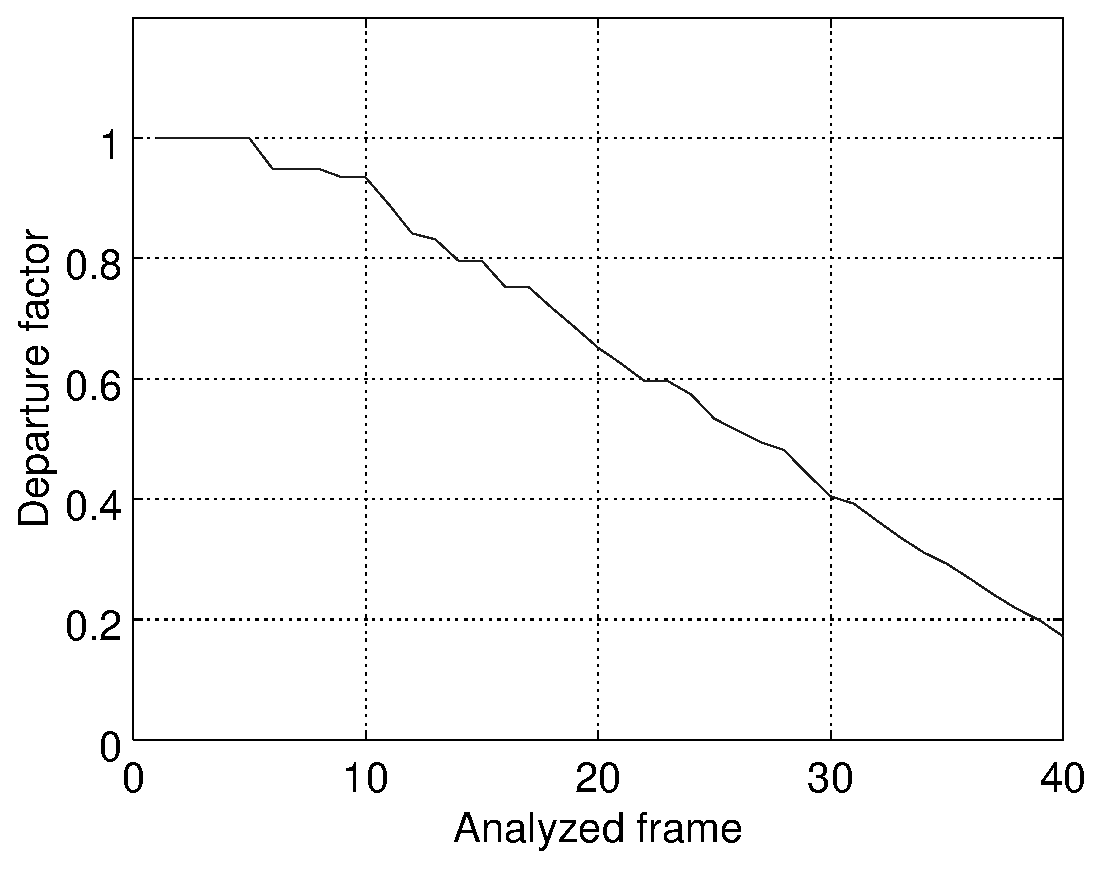
\includegraphics[width=\columnwidth]{images/grapha_b.eps}
\caption{Departure factor for each frame in the test 2.}
\label{fig:res_grapha_b}
\end{figure}

The Fig. \ref{fig:res_grapha_b} shows the departure factor in each frame
of test 2 (see the line with circles), additionally It is showed a polynomial
fitting of departure factor using a polynomial of order 4 (see the line with dots),
finally It is showed the real route of target normalized to $1.0$ for the maximum distance
(see the line with squares), as can be seen the target is approaching with a constant speed. 
If we interpret this value as the position in each sample time, 
then the departure factor describes the relative target position.
In the first image the analyzed target is at a distance $d_0$ 
and in the last image the target is at a distance of $17.18\%$ of $d_0$.
The departure distance decreases in discrete steps because the departure
factor is selected in discrete steps, if the target is
between two consecutive analysis layers (scales), the algorithm
approximates the target to the nearest layer.



The Table \ref{tab:tab1} represents the bank of images used for test 2, totally 40 images generated by POV-Ray.
The number of analyzed frames are in the first column of table, in the second column are the real distances 
between camera and target.
The percentage proportion of real distances are in third column. For example, 
the target in first frame is to $23.5$ meters from camera and it is considered the $100$\% of distance,
by other side, in the frame $40$ the target is to $4$ meters 
from camera and is $17,02$\% in relation of first frame. Next column, fourth column, 
we have the results of algorithm (departure factor), in the percentage form. 
%Note in first frame, target is $100$\% of distance and the last frame is at $17,18$\% of distance in relation of first frame.
Finally, the last column represents the error between percentage real distance and the departure factor. 
As can be seen, the error is diminishing when target is close (around 5 meters), it means that the algorithm has more precision 
when image of target is bigger because there are more information in ROI. It is a consequence of PCC, 
because in small ROI each pixel charge much information in comparative method. On other hand, if ROI is bigger,
the information is diluted around pixels; thus, the algorithm has more data to compare.
Another reason is that in the last frames $1$ pixel of target
represents a less distance in meters that $1$ pixel in the target of the first frames; consequently, the error 
of a quantity $x$ of pixels represents a less quantity of meters in the analysis of last frames.

\begin{table}[H]
\setlength{\tabcolsep}{1 pt} 
\caption{Table of comparative results}
\begin{tabular}{lllll}
Frames & Real Dist. (m) & Real Dist. (\%) & Dep. factor (\%) & Relative error (\%)\\
1 & 23.5 & 100.0 & 100.0 & 0.0 \\
10 & 19.0 & 80.85 & 93.46 & 15.60 \\
20 & 14.0 & 59.57 & 65.16 & 9.37 \\
30 & 9.0 & 38.30 & 40.46 & 5.65 \\
40 & 4.0 & 17.02 & 17.18 & 0.93
\end{tabular}
\label{tab:tab1}
\end{table}

The velocity of departure factor is shown in 
Fig. \ref{fig:res_grapha_bv}, where the velocity is calculated
to $d_0=1$ and $\Delta t=1$. The value of the departure
velocities is negative, which indicates that the
target is approaching towards the observer. Relative velocity is calculated 
using the discrete-time derivate.
If we compare test 1 and 2 to the same $\Delta t=1$, it is evident 
that the departure velocity of  test 2  is lower than test 1. 
Note target approaches more in test 2 and, consequently, departure
velocity is lower than test 1.
\begin{figure}[!hbt]
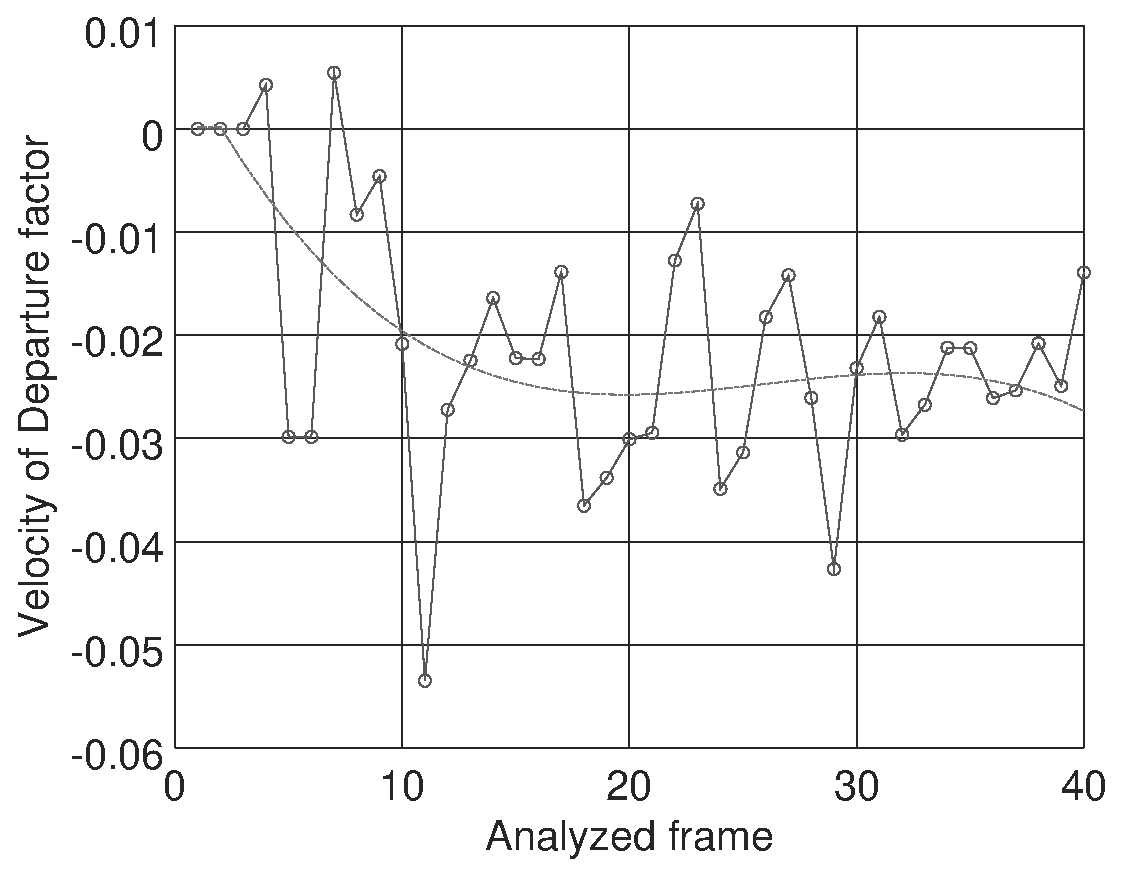
\includegraphics[width=\columnwidth]{images/graphvelocity.eps}
\caption{Velocity of departure factor for each frame in test 2.}
\label{fig:res_grapha_bv}
\end{figure}


%testes com diferentes parametros
% tabelas e graficos

\section{CONCLUSIONS}
From the presented examples,
it can be observed that one application that uses the tracking
and the departure factor is related with the risk of collision.
It is possible to estimate how of fast an object is departing.
Thus, if the  departure factor tends to zero or 
if the velocity of departure factor changes to lower negatives values every time, 
probably, there is a high risk of collision. The $PIV$ technique has presented satisfactory results. 
It can be concluded that estimating collision using velocity of departure factor, 
tracking of objects in 2 or 3 dimensions, and departure distance
relative to the first position of $ROI$. 
The simulations in both cases has given promissory results.

\addtolength{\textheight}{-12cm}

\section*{ACKNOWLEDGMENT}

We want to thank to FAPEMIG, LMT and UFLA for support given to this research.
Project number associated to this research by FAPEMIG: PIDEG37-2015.

%FAPEMIG\\
%numero de bolsa\\
%numero de projeto\\
%numero de aluno


\begin{thebibliography}{99}
	\bibitem{Bastiaans} R. J. M. Bastiaans, Cross-correlation PIV; theory, implementation and accuracy. 
        Eindhoven: Technische Universiteit Eindhoven, 2000. - EUT Report 99-W-OOl. - ISBN: 90-386-2851-X.

	\bibitem{Story} A. Story et al, PIV measurements of the velocity field of a Newtonian Fluid in a stirred tank equipped 
	with the PMT type impeller.Technical Transactions - Chemistry. 2-Ch/2014.        

	\bibitem{Xu} L. Xu, Computational fluid dynamics analysis and PIV validation of a bionic vortex flow 
	pulsatile LVAD.Technology and Health Care 23 (2015) S443?S451. DOI 10.3233/THC-150981. IOS Press, 2015.
	
        \bibitem{Miranda Neto} A. Miranda Neto et al, Image Processing Using Pearson's Correlation Coefficient: 
        Applications on Autonomous Robotics. 
        Autonomous Robot Systems (Robotica), 2013 13th International Conference on, 2013.
        
        \bibitem{Geiger} A. Geiger et al,
        Vision meets Robotics: The KITTI Dataset. International Journal of Robotics Research (IJRR), 2013, 
        doi:10.1177/0278364913491297 .
        
        \bibitem{Eugene} Y. K. Eugene and R.G. Johnston, The Ineffectiveness of the Correlation Coefficient for Image Comparisons.
        Technical Report LA-UR-96-2474, Los Alamos, 1996.
        
        \bibitem{Honegger} D. Honegger et al, Real-time Velocity Estimation based on Optical Flow and disparity matching.
         Intelligent Robots and Systems (IROS), 2012 IEEE/RSJ International Conference on Intelligent Robots and Systems.
        
        \bibitem{Breugel} F. van Breugel, K. Morgansen and M. H Dickinson, Monocular distance estimation from optic flow during
        active landing maneuvers. Bioinspiration and Biomimetics, Volume 9, Number 2. Published 22 May 2014 IOP Publishing Ltd.
        
	\bibitem{povray}  C. Cason et al.Persistence of Vision Pty. Ltd. (2017).Persistence of Vision Raytracer.
	Persistence of Vision Pty. Ltd., Williamstown, Victoria, Australia. http://www.povray.org/
	
\end{thebibliography}

\end{document}
